\newpage
\chapter{Оператори за контрол на изпълнението и потребителски функции}
\label{chapter05}

С процеса на усвояване на софтуерния продукт R всеки потребител установява, че някои команди биват повтаряни многократно. Това навежда на мисълта, че тези команди може да бъдат групирани и съхранени като програмен скрипт\index{програмен скрипт} (модел на експеримента). Основното предимство на такава организация е възможността един и същи модел да бъде използван са множество експерименти. Второто предимство е, че моделът\index{експериментален модел} може да бъде разменян между различни потребители, които работят над същата задача или сходни задачи. Езикът R е в групата на интерпретивните програмни езици, където се намира и програмният език JavaScript. За потребителите познаващи JavaScript, някои конструкции в R биха били изключително познати. 

Скриптовете на R се записват в обикновени текстови файлове с .r разширение, както примерният файл на адрес:

\begin{lstlisting}[caption=Адрес на примерен R скрипт, label=listing0074]
https://raw.githubusercontent.com/TodorBalabanov/Statistical-Data-Processing-with-R/master/code/example0001.r
\end{lstlisting}

Може да се пише с текстов редактор по избор на потребителя, но може да се използва и текстовия редактор към продукта (Фиг. \ref{figure0025}).

\begin{figure}[h!]
  \centering
  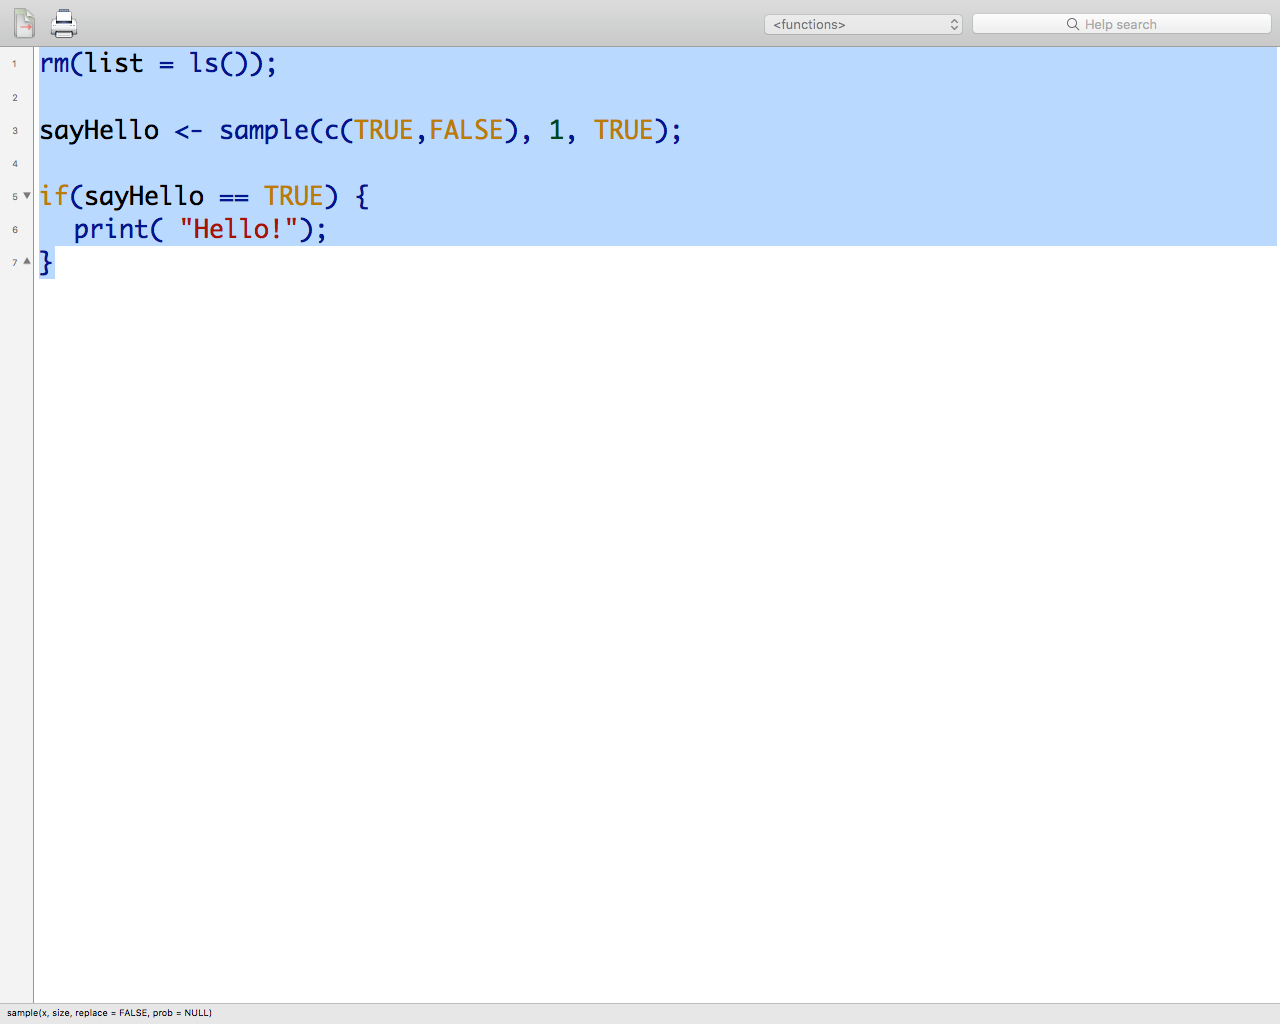
\includegraphics[width=1.0\linewidth]{pic0025}
  \caption{Текстов редактор към продукта R}
\label{figure0025}
\end{figure}
\FloatBarrier

Най-бързият начин за стартиране на скрипта\index{изпълнение на скрипт} е чрез менюто на вградения текстов редактор Edit->Execute (Фиг. \ref{figure0026}). 

\begin{figure}[h!]
  \centering
  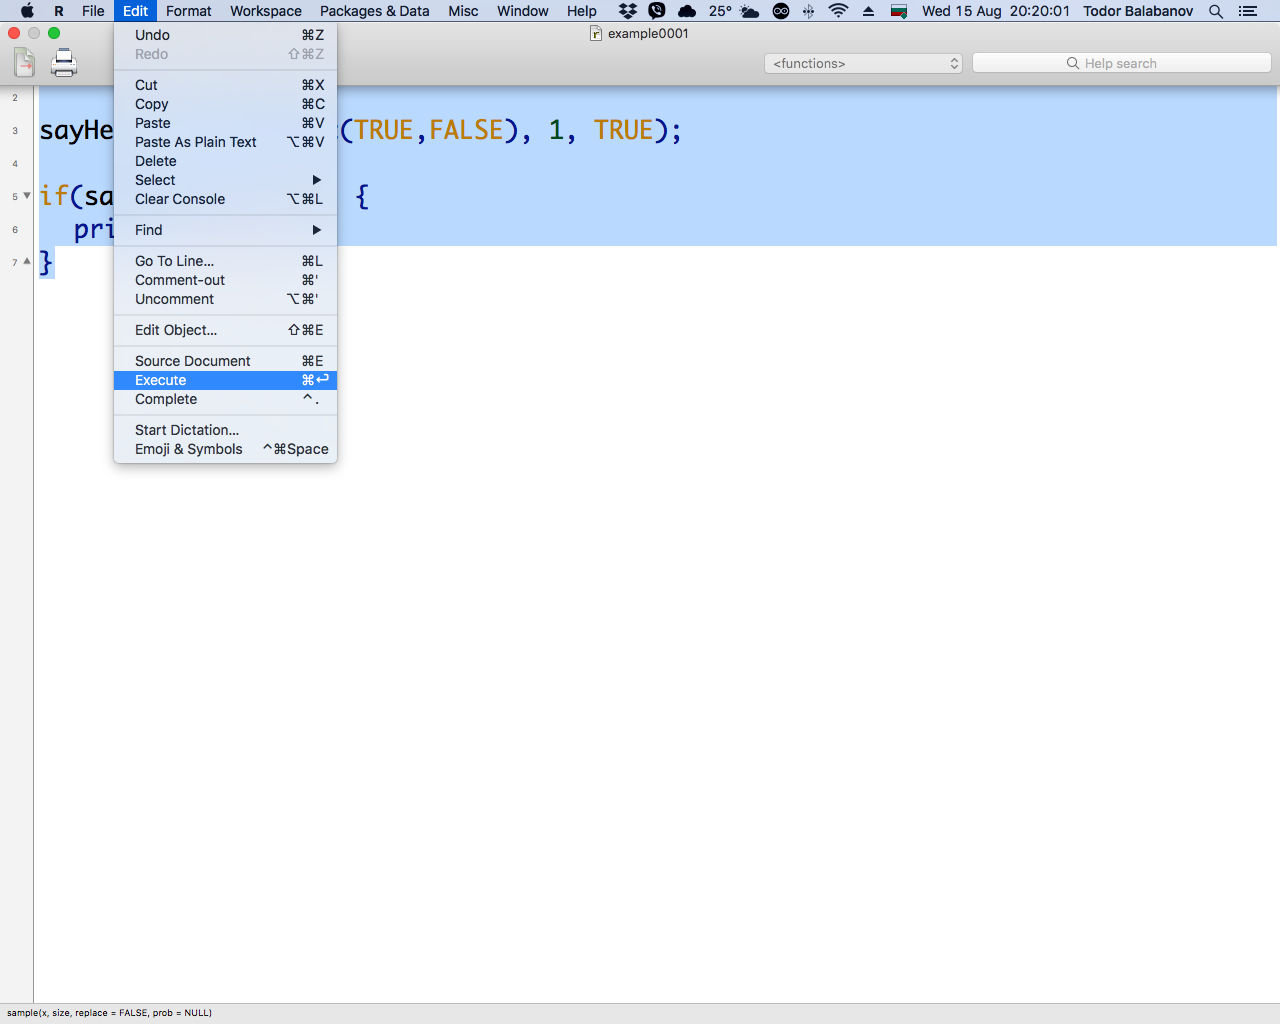
\includegraphics[width=1.0\linewidth]{pic0026}
  \caption{Стартиране на R скрипт}
\label{figure0026}
\end{figure}
\FloatBarrier

Съществено е целият текст на скрипта да бъде маркиран, тъй като командният интерпретатор е оптимизиран в режим за изпълнение на команда по команда. Когато целият скрипт е маркиран се изпълняват, една след друга, всички команди.

\begin{figure}[h!]
  \centering
  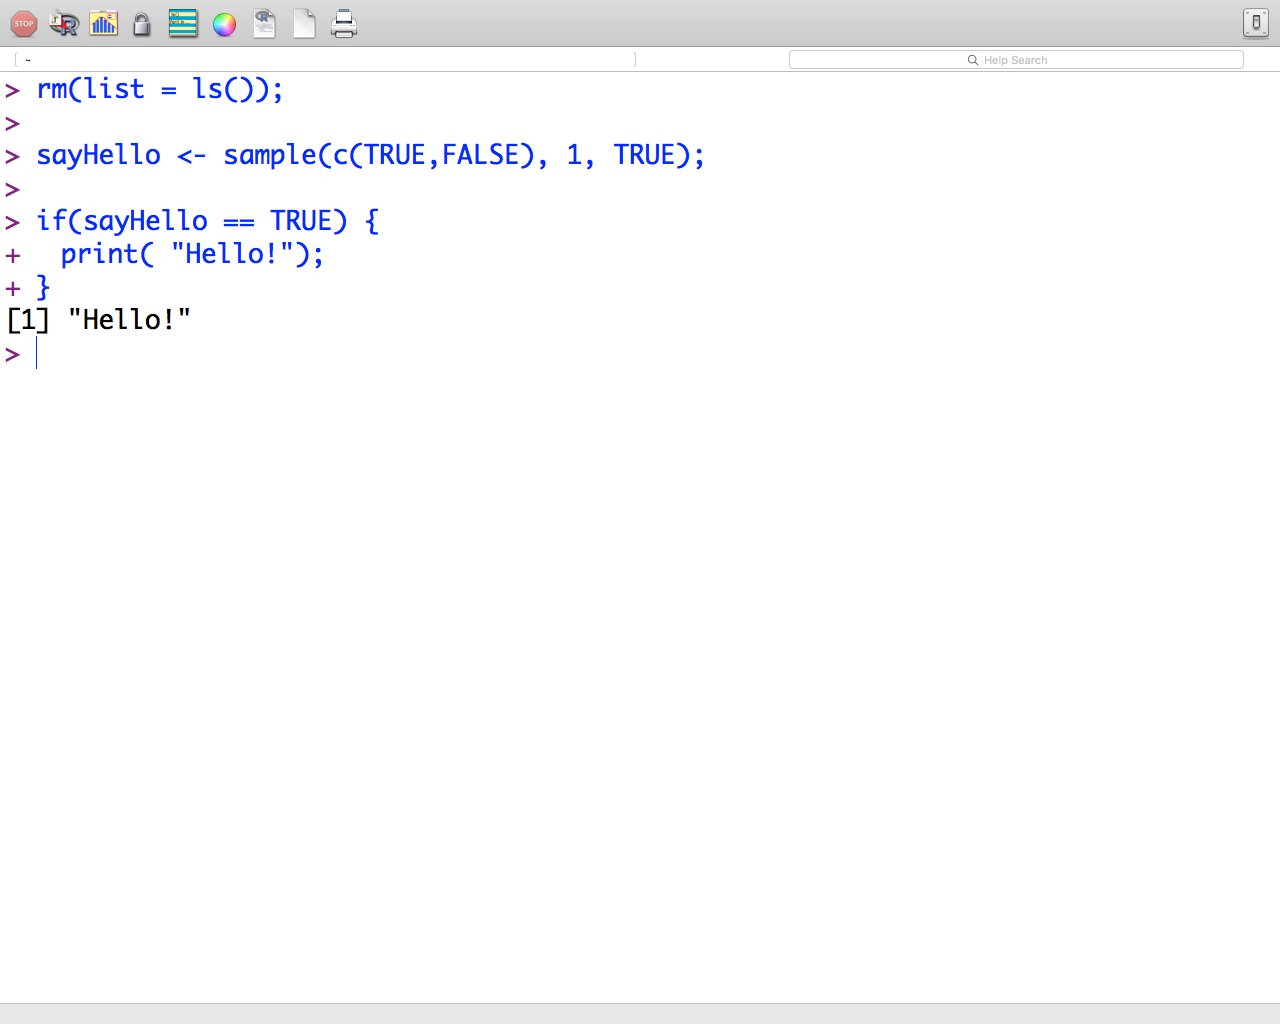
\includegraphics[width=1.0\linewidth]{pic0027}
  \caption{Резултат от изпълнението на R скрипт}
\label{figure0027}
\end{figure}
\FloatBarrier

Резултатът от изпълнението на R скрипта се наблюдава в командния интерпретатор на продукта (Фиг. \ref{figure0027}) и изглежда точно както би трябвало командите да се въведат, на ръка, ако не бяха заредени от скриптов файл.

Алтернативна възможност за стартиране на R скриптове е конзолата на операционната система. При този вариант в конзолата на операционната система се извиква приложението R, а като параметри на приложението се подава файлът съдържащ скрипта и параметър дали сесията от изпълнението на скрипта да бъде съхранена (Листинг \ref{listing0085}).

\begin{lstlisting}[caption=Изпълнение на R скрипт от конзолата на операционната система, label=listing0085]
r < ./Statistical-Data-Processing-with-R/code/example0001.r --no-save
\end{lstlisting}

При такова изпълнение се спестява зареждането на целият програмен продукт R за постоянно в оперативната памет (Фиг. \ref{figure0028}).

\begin{figure}[h!]
  \centering
  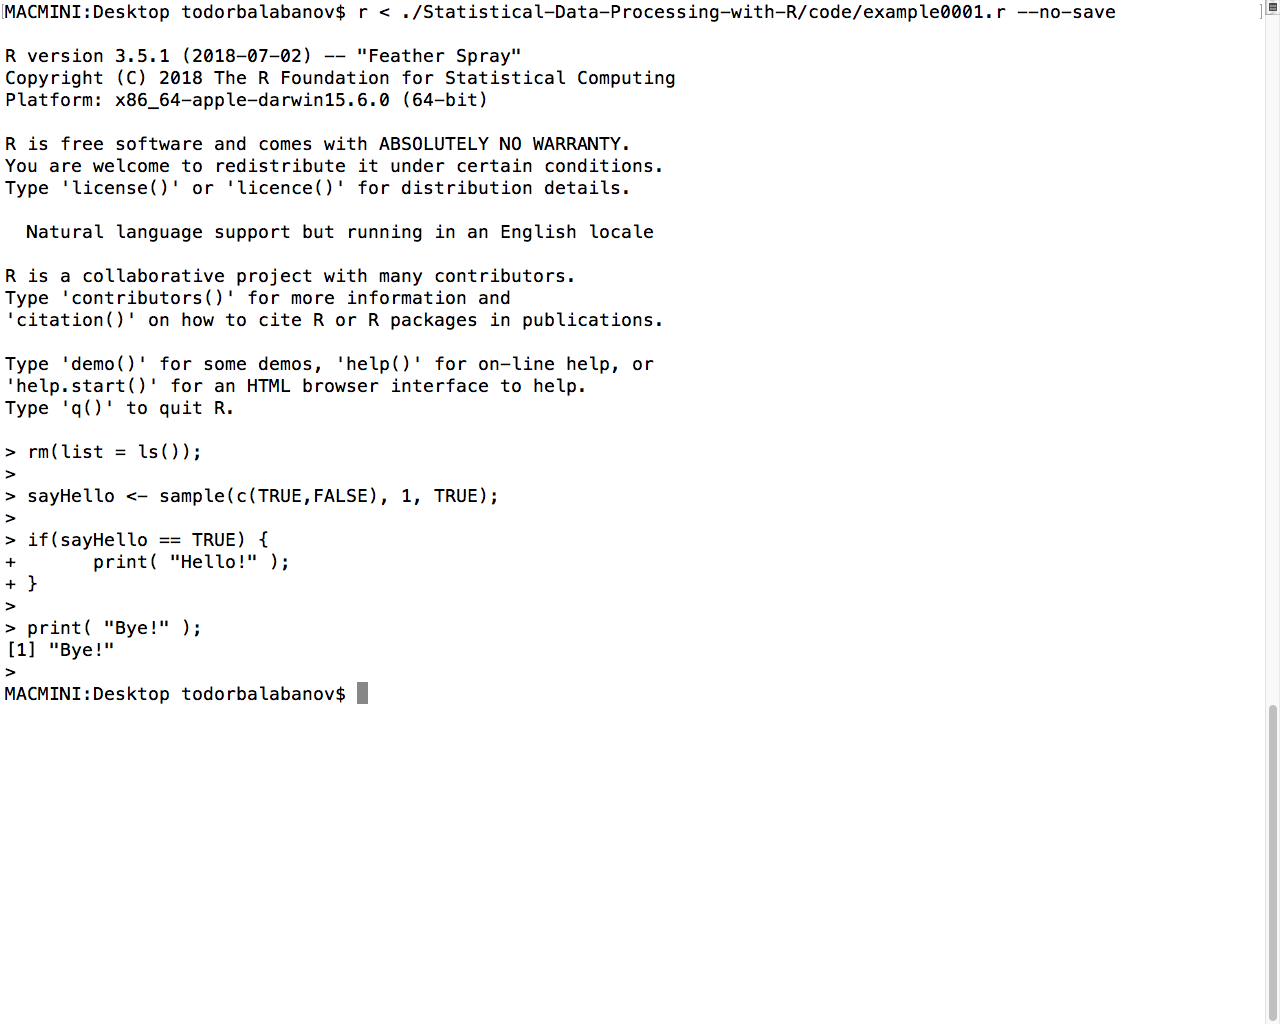
\includegraphics[width=1.0\linewidth]{pic0028}
  \caption{Резултат от изпълнението на R скрипт в конзолата на операционната система}
\label{figure0028}
\end{figure}
\FloatBarrier

Програмните скриптове се състоят от последователни инструкции, но с подходящи оператори за преход или повторение изпълнението на командите може да протече в различен от линейния ред. Тази група оператори се нарича оператори за контрол на изпълнението. Общата конструкция на операторите е заглавна част (ключова дума и условие) и тяло. 

\section{Оператори за преход}

Операторите за условен преход\index{оператори за преход} променят изпълнението на скрипта в зависимост от логическо или числено условие. От там идва и названието им. В тази група оператори попадат if, else и switch.

В заглавните части на операторите за преход може да се проверява само едно условие или да се проверяват цяла група от условия (логически изрази)\index{логически операции}. За тази цел в R има логически операции като „И“ (операции \& и \&\&) и „ИЛИ“ (операции | и ||). При дойната форма на операциите се сравнява само по една стойност от двете страни (не са векторизирани), докато при единичната форма се сравняват елемент по елемент в множества от елементи от двете страни. Поради тази причина двойната форма е полезна при if оператора, а единичната форма се изисква при ifelse конструкцията. Друга много важна разлика между единичната и двойната форма е в начина по който се изчисляват изразите от двете страни на операцията. При единичната форма задължително се изчисляват и двата операнда, независимо дали това действително е нужно. При двойната форма се изчисляват само тези операнди, които са достатъчни за да определят финалният резултат от пресмятането на логическия израз. Тази разлика в използването на логическите операции може да се окаже изключително съществена, когато операндите са функции връщащи логическа стойност. В случаите когато е ненужно някой от операндите да се изчисли, тъй като другите вече са определили резултата, то част от функциите няма да бъдат извикани. С помощта на логическите операции могат да се построят много сложни логически изрази, при които важат общите правила за приоритет на операциите, както и възможността приоритетът да се променя, чрез подходящо поставяне на скоби. 

\subsection{Оператор за условен преход}

Дори чисто исторически в програмните езици един от първите оператори за преход е оператора за условен преход (if оператор)\index{оператор за условен преход}. 

\begin{lstlisting}[caption=Оператор за условен преход if, label=listing0075]
sayHello <- sample(c(TRUE,FALSE), 1, TRUE);

if(sayHello == TRUE) {
	print( "Hello!" );
}

print( "Bye!" );
\end{lstlisting}

Операторът за условен преход използва ключовата дума if (Листинг \ref{listing0075}), а в заглавната му част се записва израз пресмятан до логическа стойност TRUE или FALSE\index{логически стойности}. Смисълът на оператора if е, че тялото му бива изпълнено единствено ако изчислението на израза в заглавната част доведе до стойност TRUE. Ако изразът в заглавната част бъде изчислено до стойност FALSE, тялото на оператора се пропуска и изпълнението на програмата продължава след него.

В примерът от листинг \ref{listing0075} променливата sayHello получава една случайна логическа стойност (TRUE или FALSE), като двете възможности за равно вероятни. На следващият ред операторът if изписва "Hello!" или го пропуска и изписва "Bye!". Скриптът трябва да се стартира няколко пъти за да се наблюдава ефекта от случайния избор на стойност за променливата sayHello.

\subsection{Алтернатива при условен преход}

В множество ситуации, освен основна алтернатива за оператора if, е необходимо да има и допълнителна алтернатива\index{алтернатива при условен преход}, която да се изпълни при резултат от логическия израз FALSE. За тази цел конструкцията на оператора if може да се разшири с добавяне на else конструкция (Листинг \ref{listing0076}).

\begin{lstlisting}[caption=Оператор за условен преход if-else, label=listing0076]
sayHello <- sample(c(TRUE,FALSE), 1, TRUE);

if(sayHello == TRUE) {
	print( "Hello!" );
} else {
	print( "Hi!" );
}

print( "Bye!" );
\end{lstlisting}
Конструкцията else е контекстно зависима и поради тази причина може да се използва единствено в комбинация с конструкцията на оператора if. В примерния код от листинг \ref{listing0076} в половината от случаите на конзолата ще се изпише "Hello!", а в другата половина "Hi!".

\subsection{Каскада от условни преходи}

Условният преход ограничава до две възможности, но практиката понякога налага да се избират повече алтернативи. В такава ситуация може да се използва каскада от if-else конструкции\index{каскада от оператори за условен преход} (Листинг \ref{listing0077}).

\begin{lstlisting}[caption=Каскада от if-else, label=listing0077]
sayHello <- sample(c(0,1,2), 1, TRUE);

if(sayHello == 0) {
	print( "Hello!" );
} else if(sayHello == 1) {
	print( "Hi!" );
} else if(sayHello == 2) {
	print( "Yoo!" );
} else {
	print( "Error!" );
}

print( "Bye!" );
\end{lstlisting}

Недостатък на каскадните проверки е, че всяко условие трябва да бъде проверявано по отделно. Каскадата може да завършва с else конструкция, но тя не е задължителна. 

R предлага ifelse оператор, който много прилича на if конструкцията в Microsoft Excel (Листинг \ref{listing0078}) и сериозно се различава от if-else оператора. Една от най-силните страни на ifelse конструкцията е, че тя е векторизирана и може да се прилага над група елементи едновременно. 

\begin{lstlisting}[caption=Функцията ifelse, label=listing0078]
ifelse(sample(c(FALSE,TRUE), 1, TRUE), "Yes", "No")

ifelse(c(1,1,0,1,0,1)==1, "Yes", "No")
\end{lstlisting}

\subsection{Оператор за многовариантен избор}

Писането на каскадни конструкции от типа if-else може да бъде твърде неудобно и поради тази причина съществува switch конструкцията\index{оператор за многовариантен избор} (Листинг \ref{listing0079}).

\begin{lstlisting}[caption=Конструкция за многовариантен избор switch, label=listing0079]
switch(sample(c("a","b","c","d","e"),1,TRUE), "a"="one", "b"="two", "c"="three", "d"="four", "other")
\end{lstlisting}

В примерния код на случаен принцип се избира една буква от пет възможни, след което се проверяват четири алтернативи и последна опция за else условие. 

Първият аргумент е стойността която ще се проверява, а след това са изброени алтернативните възможности. Последната стойност, ако не й е зададена стойност за проверка, служи за отговор, коато нито една от алтернативите не е била определена. 

\section{Оператори за цикъл}

В конвенционалните програмни езици е обичайна практика елементите на масивите и контейнерите за данни (списъци, стекове, опашки и други) да бъдат обхождани един по един с помощта на цикли. В R целта е да бъдат прилагани векторизирани операции и максимално да се избягва използването на цикли за обхождане на елементи в контейнер за данни. Въпреки това, в някои ситуации се налага използването на цикли\index{оператори за цикъл} и поради тази причина R поддържа циклите for и while. 

\subsection{Цикъл за обхождане}

Операторът for\index{цикъл за обхождане} в R представлява цикъл за обхождане на елементи във вектор, като елементът от текущата итерация е достъпен за използване в тялото на цикъла (Листинг \ref{listing0080}). 

\begin{lstlisting}[caption=Оператор за цикъл for, label=listing0080]
for(number in 1:10) { print(number); }
[1] 1
[1] 2
[1] 3
[1] 4
[1] 5
[1] 6
[1] 7
[1] 8
[1] 9
[1] 10
\end{lstlisting}

Заглавната част се състои от променлива (в случая number), ключовата дума in и вектор от възможни стойности (в случая числата от едно до десет). Векторите могат да бъдат с различен тип на елементите, примерно символни низове (Листинг \ref{listing0081}).

\begin{lstlisting}[caption=Обхождане на вектор от символни низове, label=listing0081]
for(f in c("orange", "lemon", "kiwi", "cherry")) { print(f); }
[1] "orange"
[1] "lemon"
[1] "kiwi"
[1] "cherry"
\end{lstlisting}

\subsection{Цикъл с условие за край}

Когато няма да бъде обхождано множество от елементи е по-удачно да се използва цикълът while\index{цикъл с условие за край}, който в заглавната си част съдържа логически израз, определящ условието за край на цикъла. Цикълът се върти докато логическият израз в заглавната му част се пресмята до стойност TRUE (Листинг \ref{listing0082}). 

\begin{lstlisting}[caption=Цикъл с условие за край, label=listing0082]
counter <- 1;
while(counter <= 5) { 
	print( counter ); 
	counter <- counter + 1;
}
[1] 1
[1] 2
[1] 3
[1] 4
[1] 5
\end{lstlisting}

При цикъла с условие за край, променливата която определя условията за приключване на итереациите трябва да се определи преди началото на цикъла. За да не бъде цикълът безкраен е нужно тази променлива да бъде променена, в тялото на цикъла, по такъв начин, че той да приключи изпълнението си.

\subsection{Прекъсване на циклите}

Понякога се налага определена итерация на цикъла да бъде прекъсната\index{прекъсване на цикли}. За тази цел R предлага ключовата дума next, която прекъсва текущата итерация и преминава към следващата (Листинг \ref{listing0083}).

\begin{lstlisting}[caption=Прекъсване на итерация, label=listing0083]
for(number in 1:10) { 
	if(number == 7) {
		next;
	}

	print(number);
}
[1] 1
[1] 2
[1] 3
[1] 4
[1] 5
[1] 6
[1] 8
[1] 9
[1] 10
\end{lstlisting}

В този случай пропуснатото число е седем, тъй като при седмата итерация е било изпълнено условието на оператора if и неговото тяло съдържа ключовата дума next.

В други ситуации се налага цикълът да бъде спрян изцяло и тогава се използва ключовата дума break (Листинг \ref{listing0084}).

\begin{lstlisting}[caption=Прекъсване на цикъла, label=listing0084]
for(number in 1:10) { 
	if(number == 3) {
		break;
	}

	print(number);
}
[1] 1
[1] 2
\end{lstlisting}

Двете ключови думи (next и break) са контекстно зависими конструкции и могат да се използват единствено в телата на циклите for и while. 

\section{Потребителски функции}

При писането на програмен код в съвременните програмни езици е изключително добра практика кодът да се групира в серия инструкции и те да се оформят като самостоятелна единица. За тази цел, R предлага възможността кодът да се оформя в потребителски написани функции\index{потребителски функции}. 

Оформянето на скриптовете в добре организирани и малки по размер функции е основен похват в съвременното програмиране. Такъв стил на работа позволява по-лесна поддръжка, по-лесна проверка на резултатите създавани от функцията и по-лесна преизползваемост на кода. 

Писането на функции в R малко се различава от повечето конвенционални програмни езици, но много прилича на функциите писани в JavaScript. Самата функция представлява обект, който бива присвоен на идентификатор (Листинг \ref{listing0086}).

\begin{lstlisting}[caption=Примерна потребителска функция, label=listing0086]
say.hello <- function() {
	print("Hello, World!");
}

say.hello();
[1] "Hello, World!"
\end{lstlisting}

Важно е да се отбележи, че символът точка (.) е валиден символ за съставяне на име на функцията. Това е фундаментална разлика спрямо повечето конвенционални програмни езици. Въпреки това, имената не бива да започват само с точка, тъй като обекти именувани по този начин имат по-специфична употреба. Функцията се създава с ключовата дума function\index{дефиниция на функция}, а тялото на функцията се огражда в къдрави скоби. Много добра практика е да се спазват стриктни правила за подравняване на различните конструкции, използвани като команди в тялото на функцията. Такъв стил на писане подобрява възможностите за четене програмния текст и възможностите за откриване на евентуални грешки в него. 

\subsection{Аргументи на функция}

Тъй като функциите са самостоятелно обособени групи от инструкции, то понякога е нужно към групата да бъдат подавани параметри, под формата на аргументи на функцията\index{аргументи на функция} (Листинг \ref{listing0087}). 

\begin{lstlisting}[caption=Извикване на функция с аргумент, label=listing0087]
hello.person <- function( name ) {
	print( sprintf("Hello, %s!",name) );
}

hello.person("Dessislava");
[1] "Hello, Dessislava!"
\end{lstlisting}

Променливата name е достъпна само в тялото на функцията и не може да бъде използвана извън него. 

\begin{lstlisting}[caption=Извикване на функция с повече аргументи, label=listing0088]
hello.person <- function(first, last) {
	print( sprintf("Hello, %s %s!",first,last) );
}

hello.person("Dessislava", "Gruncharova");
[1] "Hello, Dessislava Gruncharova!"

hello.person(last="Mladevnova", first="Vyara");
[1] "Hello, Vyara Mladevnova!"
\end{lstlisting}

Функциите в R позволяват викане с изброяване на параметрите по позиции или чрез явно указване кой аргумент каква стойност да получи (Листинг \ref{listing0088}).

\subsection{Аргументи с подразбираща се стойност}

В някои ситуации е удачно някои от аргументите да имат зададена стойност по подразбиране. В много от съвременните езици това се постига с едноименни функции (overloading), но в R този ефект е възможен, чрез задаване на подразбираща се стойност\index{аргументи на функция с подразбираща се стойност} (Листинг \ref{listing0089}). 

\begin{lstlisting}[caption=Извикване на функция с подразбиращи се аргументи, label=listing0089]
hello.person <- function(first, last, title="") {
	print( sprintf("Hello, %s %s %s!",title,first,last) );
}

hello.person("Zornitsa", "Radeva", "Miss");
[1] "Hello, Miss Zornitsa Radeva!"

hello.person("Todor", "Balabanov");
[1] "Hello,  Todor Balabanov!"
\end{lstlisting}

\subsection{Променлив брой аргументи}

По аналогия с програмния език C, в R са възможни функции с променлив брой аргументи, което се постига с операцията триеточие (...) в заглавната част на функцията (Листинг \ref{listing0090}). Механизмът с променлив брой аргументи\index{функции с променлив брой аргументи} е изключително полезен, но той също така води и до много сериозни програмни грешки. 

\begin{lstlisting}[caption=Функция с променлив брой аргументи, label=listing0090]
sum.up <- function(a, b, ...) {
	print( a+b );
}

sum.up(1, 2, 3, 4);
\end{lstlisting}

\subsection{Върната стойност}

Потребителските функции трябва да се пишат по такъв начин, че да функционират на принципа на черната кутия – аргументи на входа с резултат на изхода и капсулирано изчисление в тялото на функцията. За да бъде постигната тази цел, функциите в R могат да връщат стойност\index{върната стойност от функция}. По аналогия с JavaScript, в R може да се връща стойност от различен тип с ключовата дума return (Листинг \ref{listing0091}).

\begin{lstlisting}[caption=Връщане на стойност от функция, label=listing0091]
sum.up <- function(a, b, ...) {
	return(a + b);
}

print( sum.up(1,2,3,4) );
\end{lstlisting}

\subsection{Предаване на функция като аргумент}

В относително редки случаи се налага върху входните данни да бъдат извикани различни функции. В такава ситуация е важно към самата функция да бъде подаден обект от тип функция\index{функционални обекти} (Листинг \ref{listing0092}).

\begin{lstlisting}[caption=Избор на функция за извикване по време на изпълнение, label=listing0092]
do.stat <- function(values, calculation) {
	do.call(calculation, args=list(values));
}

print( do.stat(1:10,mean) );
[1] 5.5

print( do.stat(1:10,median) );
[1] 5.5

print( do.stat(1:10,sd) );
[1] 3.02765
\end{lstlisting}

В други програмни езици този ефект се постига с функционални указатели (езикът C) или функционални обекти (езикът Java).

\section*{Заключение}

Операторите за контрол на изпълнението позволяват създаването на по-сложни експериментални модели и извършването на по-задълбочени статистически изследвания. За ефективна и надеждна работа, езикът R позволява командите и операторите за контрол на изпълнението да бъдат организирани в отделни потребителски функции и файлове съдържащи програмните скриптове. 

